\section{Speech Signal Processing}

\begin{frame}
\frametitle{Analog-to-Digital Conversion}
\begin{itemize}
\item Telephony since the 1950s limits the information bandwidth to 300-3400 Hz.
\item In normal conversational speech, the frequency content is mainly between 0-8000 Hz \cite{uysal2005bandwidth}.
\item We choose sampling rate $F_s$ = $2 \times 8000$ Hz = 16000 Hz.\\(Nyquist-Shannon sampling theorem)
\end{itemize}
\end{frame}

%----------------------------------------------------------------------------------------
%	Subsection
%----------------------------------------------------------------------------------------

\begin{frame}
\frametitle{Pre-emphasis}
\begin{itemize}
\item Pre-emphasis filter is essentially an \textbf{high-pass} filter.
\vspace{15pt}
\item Voiced speech naturally have an attenuation of $\sim$ 20 dB per decade due to physiological characteristics of the speech production system \cite{picone1993signal}.
\begin{itemize}
\item compensates this natural attenuation before spectral analysis.
\end{itemize}
\item Hearing is more sensitive to the components higher than 1 kHz.
\begin{itemize}
\item caters to human perception of sound
\end{itemize}
\end{itemize}
\end{frame}

%--------------------------------------------
%--------------------------------------------

\begin{frame}
\frametitle{Pre-emphasis}
A first-order FIR filter is widely implemented, including the previous group where $\alpha = 0.95$ \cite{EVW-report}.
\begin{equation}
y[n] = x[n] - \alpha x[n-1]
\end{equation}
\end{frame}

%--------------------------------------------
%--------------------------------------------

\begin{frame}
The \textcolor{orange_matlab}{orange dash-dot line} shows that frequencies below 500 Hz are severely suppressed even though frequencies above 3 kHz are successfully amplified.

\begin{figure}[H]
\centering
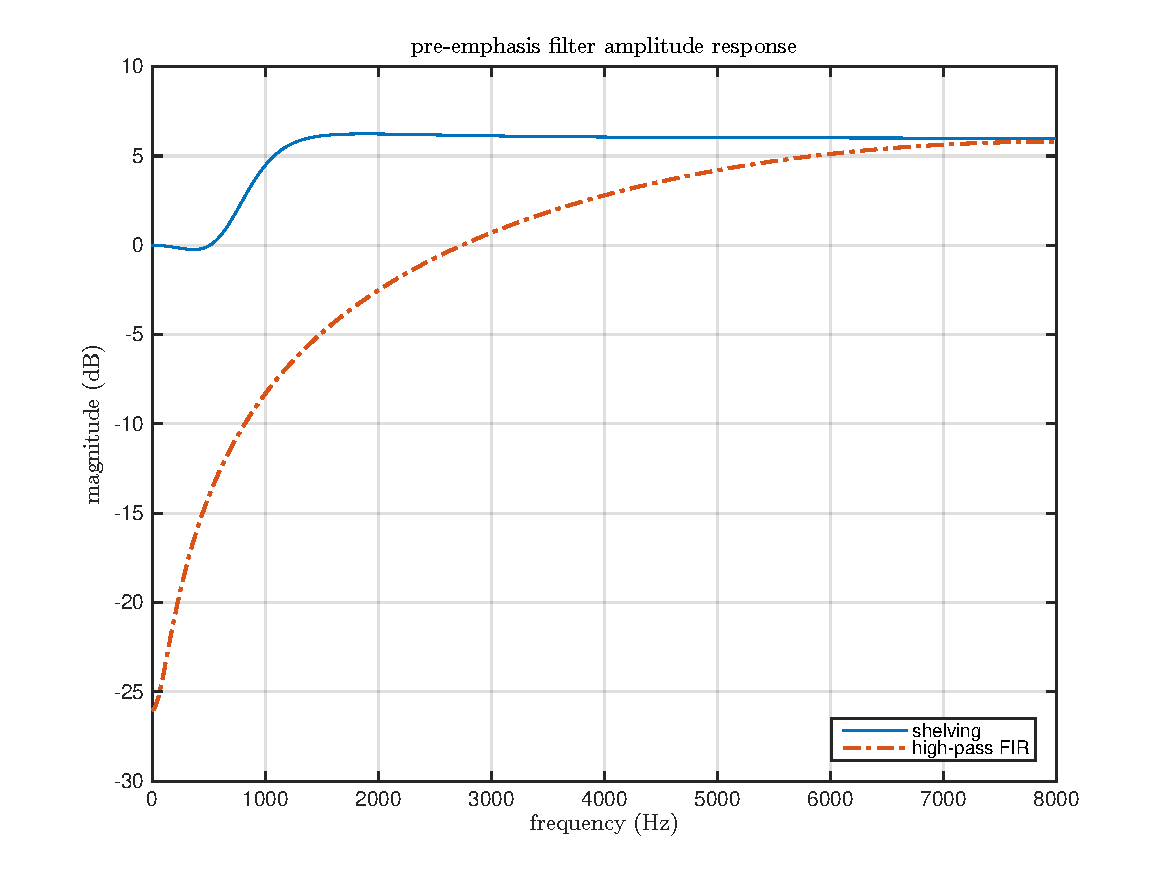
\includegraphics[width=3in, trim={0 0.6cm 0 0.6cm}, clip]{ang/pre_emphasis_filter}
\end{figure}
\end{frame}

%--------------------------------------------
%--------------------------------------------

\begin{frame}
Suggested by Professor Erik Weyer, we devised a second-order \textit{shelving filter} widely utilized in audio equalization to pre-emphasize the speech signal.

\begin{equation}
\label{shelving-filter}
y[n] = \frac{1}{a_0} \Big( b_0 x[n] + b_1 x[n-1] + b_2 x[n-3] - a_1 y[n-1] - a_2 y[n-2] \Big)
\end{equation}
where
\begin{align}
\label{shleving-coef}
&\begin{cases}
a_0 = 1\\
a_1 = -1.523796\\
a_2 = 0.649345
\end{cases}
&\begin{cases}
b_0 = 1.861856\\
b_1 = -3.102851\\
b_2 = 1.366544
\end{cases}
\end{align}
\end{frame}

%--------------------------------------------
%--------------------------------------------

\begin{frame}
Setting center frequency of transition band $F_c$ = 1000 Hz and gain $G$ = 6 dB, eventually we obtain an appropriate filter that effectively amplifies high-frequency components without attenuating low frequencies. The \textcolor{navy_matlab}{navy solid line} shows the frequency response of this shelving filter.

\begin{figure}[H]
\centering
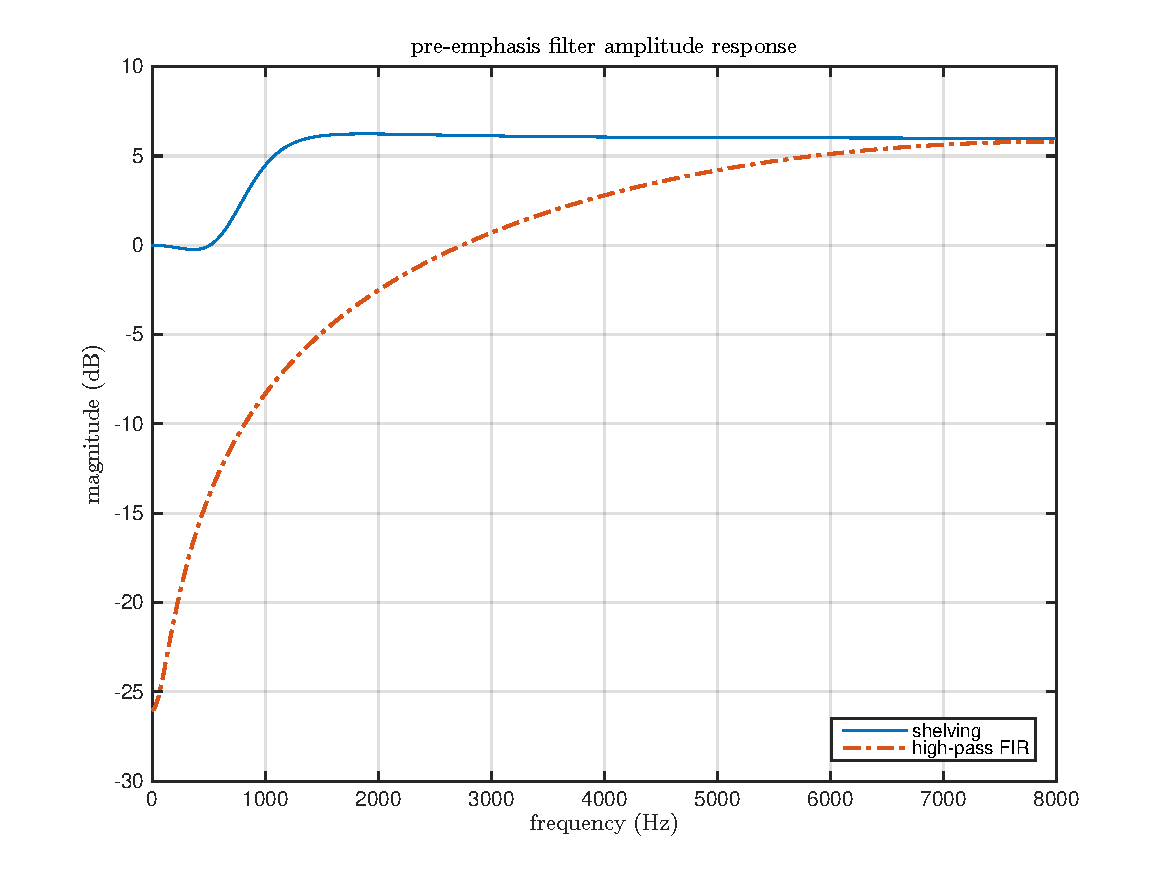
\includegraphics[width=3in, trim={0 0.6cm 0 0.6cm}, clip]{ang/pre_emphasis_filter}
\end{figure}
\end{frame}
